\newpage
\section{Entwicklung}
In diesem Kapitel wird die schrittweise Entwicklung des digitalen Zwillings für das Abfüll- und Verschließmodul der robocell-Linie dargestellt.
Ziel ist es, das physische Asset gemäß dem Konzept der \acs{aas} digital abzubilden und in ein Industrie 4.0-konformes System zu integrieren.
Abbildung \ref{fig:Entwicklungsschritte} veranschaulicht den Ablauf des zugrundeliegenden Entwicklungsprozesses.

\begin{figure}[htbp]
    \centering
    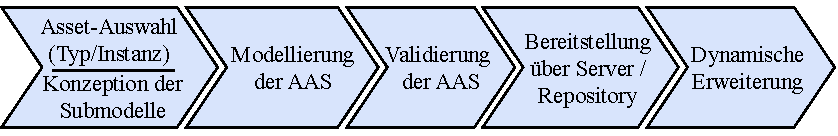
\includegraphics[width=1\textwidth]{Bilder/vorgehenEntwicklungsteil.pdf}
    \caption{Ablauf der Entwicklung des digitalen Zwillings}
    \label{fig:Entwicklungsschritte}
\end{figure}
\vspace{-1em}

Aufbauend auf einer konzeptionellen Grundlage erfolgt zunächst die statische Modellierung der \acs{aas} mithilfe des Package Explorers. 
Die resultierende Struktur wird anschließend mit einer Test Engine validiert.
Im weiteren Verlauf wird die \acs{aas} mit der Eclipse BaSyx-Plattform bereitgestellt und um dynamische Informationen ergänzt. 
Dabei werden sowohl Echtzeitdaten über \acs{opcua} als auch Zeitreihendaten über eine InfluxDB eingebunden.

Nach der Implementierung des digitalen Zwillings wird ein \acs{ki}-Modell zur Analyse und Optimierung der darin enthaltenen Daten vorgestellt und prototypisch umgesetzt.
Außerdem wird die Entwicklung von zwei exemplarischen Anwendungsfällen betrachtet.
Im ersten Anwendungsfall steht die Umsetzung eines \acs{dpp} im Vordergrund. 
Der Fokus liegt hierbei auf der strukturierten Abbildung des \acs{pcf} sowie der Implementierung differenzierter Zugriffsrechte auf die verschiedenen Bestandteile.
Im zweiten Anwendungsfall wird gezeigt, wie \acs{aas}-Instanzen automatisiert generiert und bereitgestellt werden können.

\subsection{Konzeptionierung des digitalen Zwilling}
Ziel dieses Abschnittes ist es, eine grundlegende Basis für die Erstellung des digitalen Zwillings zu schaffen.
Dabei wird untersucht, welche Daten für die Modellierung erforderlich sind, wo diese herkommen und wie sie in (standardisierten) Submodellen der \acs{aas} strukturiert werden können.
\subsubsection{Identifikation relevanter Datenquellen}
Ein digitaler Zwilling basiert immmer auf einer Vielzahl unterschiedlicher Daten, die gemeinsam ein umfassendes digitales Abbild eines Assets ermöglichen. 
Dabei werden sowohl statische Informationen (z.B. Datenblätter oder Konstruktionsdaten) als auch dynamische Daten, die während des Betriebs einer Maschine anfallen, benötigt.
Im ersten Schritt gilt es daher, alle relevanten Datenquellen zu identifizieren, die für die Modellierung des digitalen Zwillings erforderlich sind.

In industriellen Umgebungen kommen typischerweise verschiedene Systeme zur Erfassung, Verwaltung und Speicherung von Maschinendaten zum Einsatz.
Bei groninger übernimmt diese Funktion das \acs{plm}-System Agile, das eng mit dem \acs{erp}-System PSI Penta verknüpft ist.
Darin sind unter anderem Stücklisten, technische Spezifikationen, \acs{cad}-Dateien sowie allgemeine Dokumente hinterlegt, die die statische Grundlage  für den digitalen Zwilling bilden.

Neben den Informationen aus den Unternehmenssystemen spielen aber auch Laufzeitdaten, wie sie durch Sensoren oder Steuerungssysteme erzeugt werden, eine zentrale Rolle.
Da im Rahmen dieser Arbeit keine reale Maschine angebunden ist, werden diese Daten simuliert.
Hierfür kommt eine in Node.js entwickelte Anwendung zum Einsatz, die im Folgenden als Datengenerator bezeichnet wird und sowohl Prozess- als auch Betriebsdaten generiert. 

Ergänzend dazu wird ein Maschinensimulator verwendet, der einen PackML-Zustands\-automaten abbildet und typische Maschinenzustände sowie deren Übergänge simuliert. 
Beide Komponenten stehen als Docker-Container zur Verfügung und stellen die Daten über einen \acs{opcua} Server bereit, wodurch eine realitätsnahe Datenbasis geschaffen wird.
\subsubsection{Auswahl geeigneter Teilmodelle}
Aufbauend auf den zuvor betrachteten Informationsquellen gilt es nun zu entscheiden, welche Aspekte der Maschine im digitalen Zwilling, oder besser gesagt in der \acs{aas}, abgebildet werden sollen.
Im nächsten Schritt ist daher die Auswahl bzw. der Entwurf geeigneter Submodelle erforderlich, die die relevanten Informationen strukturiert bereitstellen.

Als Orientierung dienen die von der \acs{idta} bereitgestellten \acsp{smt} \cite{idtaTemplates}, die bereits viele typische Anwendungsfälle standardisiert abdecken.
Diese sind jeweils in einer Submodellspezifikation der \acs{idta} dokumentiert.
Darüber hinaus besteht jedoch auch die Möglichkeit, eigene Submodelle zu entwerfen, die gezielt auf projektspezifische Anforderungen zugeschnitten sind.
Diese können entweder vollständig neu konzipiert oder aus bestehenden Vorlagen abgeleitet werden.

Die konkrete Auswahl der Submodelle in dieser Arbeit orientiert sich hauptsächlich an typischen Industrie 4.0-Anwendungsfällen, die unter anderem auf der Website der \acs{idta} dokumentiert sind \cite{idtaUseCases}.
Diese Anwendungsfälle zeigen auf, welche Submodelle in der Praxis besonders relevant sind.
Eines der wichtigsten ist vermutlich das digitale Typenschild, da dieses häufig die erste Anlaufstelle für die Identifikation und grundlegende Informationen eines Assets darstellt.
Daneben wurden aber auch projektspezifische Anforderungen berücksichtigt, die sich aus den verfügbaren Daten sowie dem fachlichen Austausch mit Industriepartnern wie Wittenstein ergaben.

Tabelle \ref{tab:Submodelle} liefert einen Überblick über die initiale Auswahl dieser Submodelle sowie den zugehörigen Datenquellen.
Diese werden in späteren Anwendungsfällen gezielt erweitert.
Zur besseren Übersicht sind dynamische Submodelle farblich hervorgehoben, während statische Submodelle weiß hinterlegt sind.
Sofern vorhanden, verweist die Spalte Standardisierung auf das jeweils zugehörige \acs{smt} mittels der offiziellen Dokumentennummer der \acs{idta}, in der die bettrefende Version spezifiziert ist.
Die in der Spalte Vorgesehene Inhalte genannten Punkte zeigen beispielhaft auf, welche Informationen im weiteren Verlauf im digitalen Zwilling abgebildet werden sollen.

%\newpage
{\small
\begin{longtblr}[
    label = tab:Submodelle,
    entry = Submodelle mit typischen Inhalten,
    caption = {Submodelle mit typischen Inhalten}
  ]{
    colspec = {l l X[c]},
    rowhead = 1,
    vlines,
    hline{1-11} = {-}{},
    }
    \textbf{Submodell}                                   & \textbf{Typische Inhalte}                            & \textbf{Standardisierung} \\
    Typenschild                                          & \makecell[l]{Hersteller \\ Seriennummer \\ Adressinformationen}                  & IDTA 02006-3-0 \cite{SpezifikationTypenschild} \\
    Dokumentation                                     & \makecell[l]{Allgemeine Dokumente \\ Betriebsanleitungen \\ Projektzeichnungen}             & IDTA 02004-1-2 \cite{SpezifikationDokumentation} \\
    3D-Modelle                                           & Konstruktionsmodelle                & IDTA 02026-1-0 \cite{Spezifikation3DModelle}\\*
    Technische Daten                                     & \makecell[l]{Generelle Informationen \\ Technische Eigenschaften }                       & IDTA 02003 \cite{SpezifikaitonTechnischeDaten}\\*
    \acs{bom}                                     &  \makecell[l]{Strukturierte Stücklisten \\ Komponentenbeziehungen }                    & IDTA 02011-1-1 \cite{SpezifikationHierachischeStrukturen}\\*
    Wartung                                              &  \makecell[l]{Wartungsinformationen \\ Wartungsintervalle \\ }          & -  \\*
    Prozessdaten                                         &  \makecell[l]{Messwerte}             & - \\*
    Zeitreihendaten                                       &  \makecell[l]{Zeitreihen }             & IDTA 02008-1-1 \cite{SpezifikationTimeSeriesData}    \\*
    Kontrollkomponente                                   &  \makecell[l]{Betriebsmodi \\ Schnitstelle zur Automatisierung }             & - \\      
\end{longtblr}
}

Im Rahmen dieser Arbeit ist die Modellierung der \acs{aas} bzw. der verschiedenen Submodelle als Instanz vorgesehen.
Auch wenn es sich bei dem Abfüll -und Verschließmodul grundsätzlich um ein generisches Modul innerhalb der robocell-Linie handelt und somit technisch gesehen als Typ klassifiziert werden könnte, steht in diesem Projekt die exemplarische Umsetzung eines konkreten digitalen Zwillings im Vordergrund.
Dies begründet sich vor allem durch die vorgesehene Anbindung von Echtzeit- und Zeitreihendaten sowie die Abbildung einer Betriebsumgebung, was dem digitalen Zwilling einen klaren Instanzcharakter verleiht.
Außerdem unterstützt dies die spätere Demonstration der konkreten \acs{aas} im Industrie 4.0-Systemkontext.
% Im Rahmen dieser Arbeit ist die Modellierung der AAS als Instanz vorgesehen.
% Auch wenn es sich bei der robocell grundsätzlich um ein generisches Modul einer Maschinenfamil technisch um einen Typ handelt und keine
% In diesem Projekt exemplarische Umsertzung eines konkreten digitalen Zwillings im Vordergrund da echtzeitdaten un dzeitreihendaten angebunden werden und eine betriebsumgebung abgtebildet wird instanzcharackter.
% Unterstützt zudem die Demonstration der aasa im Systemkontext.


% Ein besonders wichtiges Submodell stellt die Stückliste (\acs{bom}) dar.
% Mit diesem lässt sich die hierarchische Struktur eines Assets abbilden, das aus mehreren verschachtelten Komponenten besteht.
% Für komplexe Maschinen oder Anlagen, wie im Fall der robocell, wird im Rahmen dieser Konzeption vorgesehen, einzelne ausgewählte Komponenten jeweils als eigene \acs{aas}-Instanzen zu modellieren und in der übergeordneten Haupt-\acs{aas} zu referenzieren.
% Diese werden im weiteren Verlauf als Komponenten-\acs{aas} bezeichnet.
% Auf diese Weise soll eine höhere Modularität und Wiederverwendbarkeit erreicht werden.

% Zur Verdeutlichung der zugrunde liegenden Architektur sowie der Beziehungen zwischen den identifizierten Datenquellen, \acs{aas} und Submodellen dient Abbildung~\ref{fig:konzeptionierungAAS}. 
% Die \acs{aas} der robocell bildet dabei das zentrale digitale Abbild, in das die relevanten Informationen aus den in diesem Kapitel beschriebenen Submodellen integriert werden sollen.

% \begin{figure}[htbp]
%     \centering
%     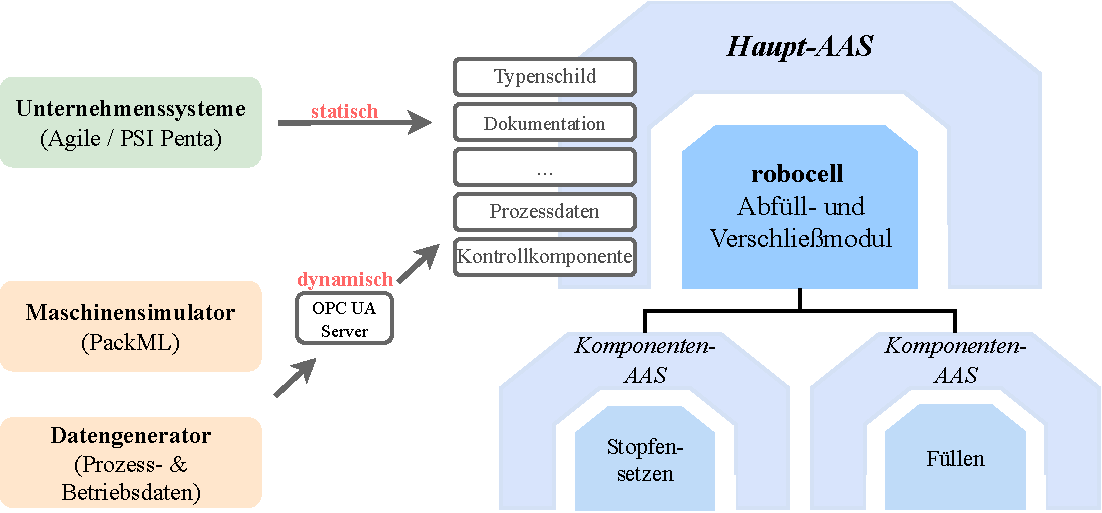
\includegraphics[width=1\textwidth]{Bilder/Konzeptionierung/konzeptionierungNeu.pdf}
%     \caption{\acs{aas}-Konzept der robocell}
%     \label{fig:konzeptionierungAAS}
% \end{figure}

\subsection{Modellierung mit der AAS}
In diesem Abschnitt wird beschrieben, wie die zuvor ausgewählten Submodelle in eine \acs{aas} integriert und mit konkreten Daten sowie semantischen Informationen angereichert werden können.
Dabei wird erläutert, wie eine \acs{aas} von Grund auf modelliert, schrittweise mit Inhalten gefüllt und abschließend gespeichert bzw. exportiert werden kann.  

Die Umsetzung erfolgt mithilfe des Package Explorers, der eine intuitive Modellierung aller relevanten Elemente der \acs{aas} ermöglicht und so den strukturierten Aufbau eines digitalen Zwillings unterstützt.
Außerdem wird gezeigt, wie sich die erstellte \acs{aas} mit einer Test Engine auf eine korrekte und vollständige Struktur überprüfen lässt.

\subsubsection{Praktische Umsetzung mit dem Package Explorer}

Die Modellierung beginnt mit dem Erstellen eines neuen \acs{aas}-Pakets im Package Explorer.
Dieses dient als Container für die digitalen Inhalte eines Assets.  
In der geöffneten Umgebung lässt sich eine neue \acs{aas} anlegen, die sowohl allgemeine als auch assetspezifische Daten enthält. 
Abbildung~\ref{fig:NeuesAASPaket} zeigt den initialen Aufbau im Package Explorer, der im weiteren Verlauf sukzessive um Submodelle und deren Inhalte erweitert wird.
Dateien, wie ein Titelbild für die robocell können dabei bereits zu Beginn in die \acs{aas}-Umgebung eingebettet werden und sind ein integraler Bestandteil des digitalen Zwillings.

Darin müssen zunächst die Metadaten der \acs{aas} sowie des zugehörigen Asset spezifiziert werden.
Neben der Auswahl des Asset-Typs ist insbesondere die eindeutige Identifikation von zentraler Bedeutung.
Das Asset selbst wird über eine globalAssetId referenziert, während die \acs{aas} eine eigene ID und eine idShort erhält.
Diese vereinfachen nicht nur den späteren Austausch der \acs{aas}, sondern ermöglichen auch deren systemweites Auffinden innerhalb eines Industrie-4.0-Ökosystems.
Für erste Modellierungszwecke empfiehlt es sich, auf automatisch generierte Beispiel-IDs zurückzugreifen, die direkt im Package Explorer erzeugt werden können.

% \vspace{-1em}
\begin{figure}[htbp]
    \centering
    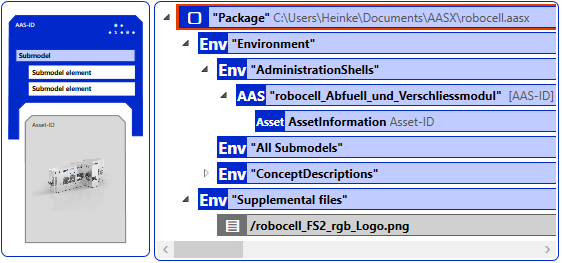
\includegraphics{Bilder/ModellierungAAS/Final/NeuesAASPaket.PNG}
    \caption{AAS-Paket im Package Explorer}
    \label{fig:NeuesAASPaket}
\end{figure}


\subsubsection*{Strukturierung durch Submodelle}
\vspace{-0.5em}

Im nächsten Schritt müssen die benötigten Submodelle zur \acs{aas} hinzugefügt werden.
Diese lassen sich entweder als Instanz, Typ oder auch Template anlegen, was eine flexible Modellierung je nach Anwendungsfall ermöglicht.
Jedes Submodell erhält dabei wie die \acs{aas} auch eine eindeutige ID, über die diese später identifiziert werden können.
Zusätzlich können optionale Administrationsinformationen angegeben werden, wie beispielsweise die Versionsnummer oder der Name des Autors.

Beim Erstellen eines Submodells ist dieses zunächst leer. 
Die Modellierung erfolgt durch das schrittweise Hinzufügen von Submodellelementen.
Tabelle~\ref{tab:Submodellelemente} gibt einen Überblick über die wichtigsten Submodellelemente, die im Package Explorer zur Verfügung stehen.

% \vspace{-0.5em}
{\small
\begin{longtblr}[
    label = tab:Submodellelemente,
    entry = Submodellelemente im Package Explorer,
    caption = {Submodellelemente im Package Explorer nach \cite{SpezifikationPart1}},
  ]{
    colspec = {l l X[l]},
    cell{1}{1} = {c=2}{},
    cell{2}{1} = {r=6}{c},
    cell{2}{1} = {bg=babyblue},
    cell{8}{1} = {r=6}{c},
    cell{8}{1} = {bg=babyblue},
    rowhead = 1,
    vline{1,3,4,5} = {-}{},
    vline{2} = {-}{},
    hline{1-2,8,14} = {-}{},
    hline{3-8,9-13} = {2-3}{}, 
    row{1} = {bg=tableHeader},
    }
    \textbf{\makecell[l]{Submodellelement}}& & \textbf{Beschreibung}\\
    \begin{sideways}DataElement\end{sideways}   &Blob & Binärdatei                                                                   \\
    &\makecell[l]{File} & \makecell[l]{Verlinkte oder eingebettete Datei mit \\ eindeutigem MIME-Type}                                                                 \\
    &\makecell[l]{MultiLanguage-\\Property} & Property mit mehrsprachigen Inhalten                              \\
    &Property & Einfaches Merkmal mit festem Datentyp                    \\
    &Range & Wertebereich mit Minimal- und Maximalwert                                                                  \\
    &\makecell[l]{Reference-\\Element} & Verweis auf interne oder externe Elemente                                     \\
    \begin{sideways}SubmodelElement\end{sideways} &Capability & \makecell[l]{Fähigkeit eines Assets, etwas bewirken \\ zu können (ohne konkrete Umsetzung)}                                                            \\
    &Entity & \makecell[l]{Einzelne Komponente (Asset) innerhalb \\ einer übergeordneten AAS  }                                                              \\
    &Operation & \makecell[l]{Funktion mit Ein- und Ausgabeparametern, die \\ von einem System ausgeführt werden kann}                                                               \\
    &\makecell[l]{Relationship-\\Element} & \makecell[l]{Beziehung zwischen zwei Elementen \\(sowohl intern als auch extern möglich)}                                   \\
    &\makecell[l]{Submodel-\\ElementList (\acs{sml})} & \makecell[l]{Geordnete Liste verschiedener Submodellelemente}                                 \\
    &\makecell[l]{SubmodelElement-\\Collection (\acs{smc})} & Sammlung von Submodellelementen                           \\
\end{longtblr}
}
\vspace{-0.5em}

Gemäß der Metamodellspezifikation \cite{SpezifikationPart1} wird zwischen DataElements und SubmodelElements unterschieden.
DataElements bilden stets die unterste Ebene im Modell. Sie enthalten konkrete Informationen wie Werte oder Dateien und können keine weiteren Elemente enthalten.
SubmodelElements hingegen sind komplexere Strukturen die wiederum als Container für untergeordnete Elemente dienen.

Submodellelemente erhalten im Gegensatz zu Submodellen keine eigene ID, sondern werden über ihre idShort eindeutig referenziert.
Diese muss innerhalb eines Submodells einzigartig sein.
Eine Ausnahme bilden \acsp{sml}, in denen die enthaltenen Elemente nicht über eine idShort, sondern nur über ihre Position (Index) identifiziert werden.

Alternativ zur manuellen Modellierung können die im Rahmen der Konzeption ausgewählten \acsp{smt} verwendet werden, wie sie in Tabelle~\ref{tab:Submodelle} aufgeführt sind.
Diese stammen beispielsweise aus dem offiziellen Repository der \acs{idta} \cite{idtaTemplates} und lassen sich als AASX-Dateien importieren.
Im Package Explorer erfolgt dies über ein sogenanntes Auxiliary AAS, das als sekundäre Umgebung zur Template-Verwaltung dient.

Die importierten Templates enthalten eine strukturierte Vorlage mit typischen Submodellelementen und reduzieren somit den Modellierungsaufwand erheblich.
Auch unternehmensspezifische Ableitungen lassen sich darauf aufbauend erstellen.
Ein vertiefter Ansatz zur Template-Nutzung findet sich in Kapitel~\ref{chap:ErstellenvonSubmodelTemplates}.

Nach dem Strukturaufbau können konkrete Inhalte wie Werte, Dokumente oder Referenzen eingepflegt werden.
Dies beschränkt sich jedoch auf statische Submodelle wie Technische Daten oder Dokumentation.
Dynamische Inhalte, etwa Betriebsdaten werden nicht direkt im Package Explorer gepflegt, sondern über externe Datenquellen (z.B. Maschinensimulator oder Datengenerator) zur Laufzeit angebunden.

Abbildung \ref{fig:SubmodellTypenschild} zeigt den strukturellen Aufbau anhand eines Auschnitts des statischen Submodells Typenschild mit bereits eingetragenen Werten.

\begin{figure}[htbp]
    \centering
    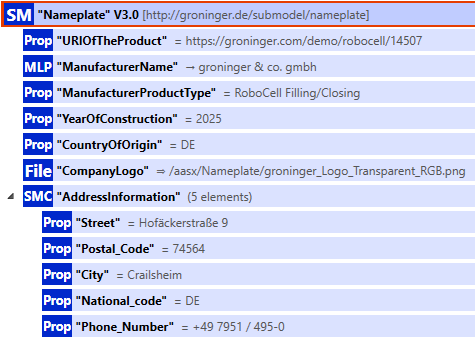
\includegraphics{Bilder/ModellierungAAS/Final/SubmodellErweitert.PNG}
    \caption{Package Explorer: Ausschnitt Submodell Typenschild}
    \label{fig:SubmodellTypenschild}
\end{figure}

\subsubsection*{Semantische Beschreibung mit Concept Descriptions}
\vspace{-0.5em}

Für die semantische Beschreibung von Submodellen und Submodellelementen innerhalb der \acs{aas} ist die Vergabe von semanticId-Referenzen essenziell.
Jede semanticId verweist auf eine zugehörige \acs{cd}, die die Bedeutung des referenzierten Elements eindeutig und maschinenlesbar beschreibt.
Im Package Explorer lassen sich solche Concept Descriptions manuell anlegen und verwalten.
Dabei steht eine vordefinierte Eingabemaske zur Verfügung, die sich an dem in Part 3a: Data Specification - IEC 61360 \cite{SpezifikationPart3a} vordefinierten Datenmodell für semantische Beschreibungen orientiert.

Die Grundstruktur dieser Vorlage ist bei allen Elementen der \acs{aas} gleich.
Allerdings unterscheiden sich je nach Elementtyp die verpflichtenden und empfohlenen Felder.
Das bedeutet, dass für verschiedene Elemente (z.B. Property oder Relationship) jeweils unterschiedliche Felder als zwingend erforderlich gelten, während andere optional oder gar nicht vorgesehen sind.
Die Struktur wird im Folgenden am Beispiel einer Property für die physikalische Größe Frequenz dargestellt.

\begin{tcolorbox}[colframe=black, colback=white, boxrule=0.8pt, arc=4pt, left=8pt, right=8pt, top=8pt, bottom=8pt]
\noindent
\begin{minipage}[t]{0.48\textwidth}
\begin{description}[style=unboxed,leftmargin=3cm,labelsep=0.2cm]
  \item[preferredName:] Frequency \mandatory
  \item[shortName:] freq \recommended
  \item[unit:] Hz \recommended
  \item[unitId:] IEC ... \recommended
  \item[sourceOfDefinition:] - \optional
  \item[symbol:] f \optional
  \item[dataType:]REAL\_MEASURE \mandatory
\end{description}
\end{minipage}%
\hfill
\begin{minipage}[t]{0.48\textwidth}
\begin{description}[style=unboxed,leftmargin=3cm,labelsep=0.2cm]
  \item[definition:] Nominal frequency ... \recommended
  \item[valueFormat:] f \optional
  \item[valueList:] \notused
  \item[value:] 50 \mandatory
  \item[valueId:] VAL001 \optional
  \item[levelType:] \notused
\end{description}
\end{minipage}
\end{tcolorbox}

\begin{tcolorbox}[legendbox]
\mandatory\ Pflichtfeld \quad
\recommended\ Empfohlen \quad
\optional\ Optional \quad
\notused\ Nicht vorgesehen
\end{tcolorbox}

Alternativ können auch externe Standards referenziert werden. 
Der Package Explorer unterstützt diesen Ansatz durch eine erweiterte Funktionalität, mit der sich vorgefertigte ECLASS-Kataloge direkt in das Tool importieren lassen. 
Nach dem Import können die enthaltenen Objekte durchsucht, ausgewählt und den entsprechenden Submodellen oder Submodellelementen zugewiesen werden. 
Die semantische Verknüpfung erfolgt dabei über eine \acs{irdi}, die das jeweilige Konzept eindeutig identifiziert \cite{eclass_irdi}. 

Wird ein solcher Standard referenziert, legt der Package Explorer automatisch eine \acs{cd} an.
Diese folgt, wie bei der manuellen Erstellung, dem in IEC~61360 definierten Datenmodell.  
So sind die semantischen Informationen auch lokal im Modell verfügbar und konsistent strukturiert.
Technisch betrachtet wäre jedoch auch eine rein externe Referenz ausreichend, da die entsprechenden Elemente bereits vollständig in den jeweiligen Katalogen enthalten sind.

Die Nutzung etablierter externer Standards ist grundsätzlich zu bevorzugen, da sie nicht nur den Modellierungsaufwand erheblich reduziert, sondern auch die Interoperabilität zwischen verschiedenen Systemen und Anwendungen deutlich verbessert.

\subsubsection*{Exportmöglichkeiten im Package Explorer}
\vspace{-0.5em}
Nach Abschluss der Modellierung lässt sich die erstellte \acs{aas} in verschiedenen Formaten exportieren.
Das bevorzugte Format in diesem Projekt ist das AASX-Format, das sich als standardisierte Austauschform für die \acs{aas} etabliert hat.
Es enthält alle modellierten Inhalte, einschließlich eingebetteter Dateien wie Bilder oder Dokumente, und eignet sich daher besonders für die Weitergabe einer Typ-1-\acs{aas}.

Alternativ kann die \acs{aas} auch als \ac{json}- oder \ac{xml}-Datei gespeichert werden.
Diese Formate beeinhalten allerdings ausschließlich die strukturierte Beschreibung der \acs{aas}, eignen sich jedoch besonders für die Nutzung in \acsp{api} oder zur Anbindung an bestehende Softwaresysteme.

Zusätzlich unterstützt der Package Explorer auch den gezielten Export einzelner Submodelle oder Concept Descriptions.
Diese lassen sich seperat, etwa als JSON-Datei abspeichern und können so gezielt in anderen \acs{aas}-Projekten wiederverwendet werden.

% \subsubsection{Abbildung hierarchischer Strukturen und Beziehungen}
% Zur Abbildung hierarchischer Strukturen, insbesondere im Submodell \acs{bom}, werden sogenannte Entities verwendet. 
% Eine Entitie repräsentiert dabei ein untergeordnetes Asset innerhalb der Gesamtstruktur. 
% Grundsätzlich lassen sich zwei Typen unterscheiden. 
% CoManagedEntities besitzen keine eigene \acs{aas} und werden innerhalb der AAS der übergeordneten Hauptkomponente mitverwaltet. 
% SelfManagedEntities hingegen, wie sie im Rahmen der Konzeption dieser Arbeit vorgesehen sind, verfügen über eine eigene \acs{aas} und können somit unabhängig verwaltet und referenziert werden. 
% Die Identifikation erfolgt über die jeweils zugewiesene globalAssetId.

\subsubsection{Validierung}
Im Anschluss an die Modellierung der \acs{aas} sollte eine Überprüfung der Konformität erfolgen.
Hierzu kann eine von der \acs{idta} bereitgestellte Test Engine \cite{TestEngine} eingesetzt werden. 
Diese lässt sich direkt mit pip, dem Paktemanager von Python, installieren und anschließend über die Kommandozeile nutzen.

Mit dem Befehl 
\tcbox[inlinebox]{{aas\_test\_engine check\_files}} 
kann beispielsweise die Validierung der zuvor erstellten \acs{aas} gestartet werden.
Unterstützt werden sowohl AASX- als auch JSON-Dateien.
Dabei wird zunächst geprüft, ob diese formal korrekt aufgebaut sind, insbesondere hinsichtlich der internen Struktur und ihrer Beziehungen.
Anschließend erfolgt die Kontrolle der enthaltenen \acs{aas} gegen die Metamodell-Spezifikationen der \acs{idta} (Teil~1 \cite{SpezifikationPart1} und 3a \cite{SpezifikationPart3a}).
Zuletzt erfolgt ein Abgleich der Submodelle mit den zugehörigen Templates, sofern diese für das jeweilige Submodell definiert wurden.

Treten bei der Validierung formale oder semantische Fehler auf, beispielsweise durch fehlende Referenzen oder ungültige IDs, gibt die Test Engine eine detaillierte Fehlermeldung in der Konsole aus. 
Diese Hinweise geben Aufschluss darüber, an welcher Stelle die Struktur bzw. der Inhalt der AASX-Datei fehlerhaft ist, und ermöglichen so eine gezielte Korrektur der betroffenen Elemente. 
Werden im gesamten Prüfprozess hingegen keine Fehler oder Abweichungen festgestellt, bestätigt die Test Engine die erfolgreiche Validierung.

\subsection{Technische Integration}
Im Anschluss an die Konzeption und Modellierung des digitalen Zwillings liegt der Fokus dieses Kapitels auf der technischen Integration der zuvor erstellten \acs{aas} in eine Industrie-4.0-kompatible Umgebung.
Dabei wird unter anderem gezeigt, wie die statisch modellierte Typ-1-\acs{aas} mithilfe des AASX Server Blazor beziehungsweise vorzugsweise der Eclipse BaSyx-Plattform in eine Typ-2-\acs{aas} überführt und systemseitig bereitgestellt werden kann.
Ergänzend dazu wird beschrieben, wie die \acs{aas} um dynamische Inhalte erweitert werden kann.
Dies umfasst die Integration von Echtzeitdaten über \acs{opcua} sowie die Einbindung und Visualisierung externer Zeitreihendaten mithilfe von InfluxDB und Telegraf.

\subsubsection{Bereitstellung der \acs{aas}}
\label{sec:bereitstellungAAS}
Für die Bereitstellung als Typ-2-\acs{aas} stehen verschiedene Open-Source-Lösungen zur Verfügung. 
Eine besonders einsteigerfreundliche Option stellt der AASX Server Blazor \cite{AASXServer} dar.
Er bildet das serverseitige Gegenstück zum Package Explorer und verfügt ebenfalls über eine grafische Benutzeroberfläche zur Visualisierung von \acs{aas}-Paketen.
Über eine HTTP-Schnittstelle können die beiden Anwendungen miteinander verbunden werden.
Dadurch lassen sich AASX-Dateien ohne zusätzlichen Konfigurationsaufwand direkt aus dem Package Explorer heraus auf den Server übertragen und bereitstellen.
Ebenso können auf dem Server gespeicherte \acs{aas} über den Explorer eingesehen und bearbeitet werden.
Die enge Verzahnung beider Komponenten ermöglicht somit eine unkomplizierte Bereitstellung und Verwaltung von \acs{aas}-Paketen und eignet sich besonders für erste Testszenarien oder prototypische Anwendungen.

Für komplexere Anwendungsszenarien, insbesondere solche mit Anforderungen an Echtzeitfähigkeit sowie an flexible und erweiterbare Submodelle, stößt der AASX Server Blazor jedoch an seine funktionalen und architektonischen Grenzen. 
So fehlen beispielsweise Schnittstellen zur Anbindung dynamischer Datenquellen sowie Möglichkeiten zur Skalierung und zur verteilten Systemintegration.
Aus diesem Grund wird im weiteren Verlauf dieses Projekts die Eclipse BaSyx-Plattform eingesetzt.
Durch ihre modulare Architektur und die klare Trennung verschiedener Komponenten wie den Registries oder den Repositories bietet sie eine deutlich flexiblere Grundlage für die Umsetzung anspruchsvoller Industrie 4.0-Szenarien.

Die einfachste Möglichkeit, BaSyx zu installieren, besteht in der Nutzung von Docker.
Alle benötigten Komponenten stehen als vorgefertigte Images öffentlich über den Docker Hub \cite{BaSyxDockerHub} zur Verfügung. 
Alternativ kann der Quellcode auch von GitHub \cite{BaSyxGithub} bezogen werden, um einzelne Komponenten individuell anzupassen oder zu erweitern.
Die verschiedenen Services, darunter die \acs{aas} Environment, Registries für \acs{aas} und Submodelle, der Discovery Service, sowie die MongoDB als persistenter Speicher, können zentral in einer docker-compose.yml-Datei verwaltet werden.
Die Konfiguration erfolgt in der Regel über Umgebungsvariablen oder seperate Konfigurationsdateien, die in der docker-compose.yml referenziert werden.
% Mit dem Befehl docker compose up lassen sich anschließend alle Komponenten gemeinsam starten.

Nach erfolgreichem Start der BaSyx-Umgebung stehen verschiedene Möglichkeiten zur Verfügung, um eine \acs{aas} bereitzustellen und in das System zu integrieren. 
Welche Methode dabei zum Einsatz kommt, hängt stark von den jeweiligen Anforderungen und Rahmenbedingungen des Anwendungsszenarios ab.
Nachfolgend werden drei ausgewählte Ansätze zur Bereitstellung näher betrachtet.

\vspace{0.5em}
\noindent\textbf{A. Volume}\\
Eine besonders einfache Variante besteht darin, eine AASX-Datei in ein gemountetes Volume der AAS Environment abzulegen.
Ein Volume ist ein persistentes Speicherverzeichnis auf dem Host-System, das mit einem Verzeichnis innerhalb eines Docker-Containers verknüpft ist.
Es ermöglicht die dauerhafte Speicherung von Daten, unabhängig vom Lebenszyklus des Containers.
In der von Eclipse BaSyx bereitgestellten Docker-Umgebung ist ein entsprechendes Volume in der Regel bereits vorkonfiguriert.

Beim Neustart der AAS Environment wird die AASX-Datei automatisch erkannt, registriert und in das BaSyx-System eingebunden.
Die dabei erzeugten Daten, darunter Informationen zu \acs{aas}, Submodellen, Concept Descriptions sowie Registrierungsdaten, werden in verschiedenen Tabellen der angebunden MongoDB gespeichert.
Dies gewährleistet, dass alle relevanten Daten persistent erhalten bleiben, selbst dann, wenn die ursprüngliche AASX-Datei später wieder aus dem Volume entfernt wird.

\vspace{0.5em}
\noindent\textbf{B. AAS Web UI}\\
Alternativ kann die Bereitstellung auch direkt über die AAS Web UI erfolgen.
Über die Benutzeroberfläche kann eine AASX-Datei manuell importiert werden, wodurch sie direkt im laufenden System registriert und eingebunden wird.
Diese Methode eignet sich besonders gut für Tests oder kleinere Anpassungen, da eine \acs{aas} auf diese Weise schnell und ohne direkten Zugriff auf das zugrunde liegende Dateisystem eingebunden werden kann.

\vspace{0.5em}
\noindent\textbf{C. REST-API}\\
Die flexibelste, jedoch auch technisch anspruchsvollste Methode zur Bereitstellung einer \acs{aas} ist die manuelle Registrierung über die \acs{rest}-\acs{api}. 
Dabei kann nicht einfach eine AASX-Datei hochgeladen werden. 
Stattdessen müssen die AAS, ihre Submodelle sowie deren Beziehungen explizit über die bereitgestellten Schnittstellen des BaSyx-Systems erstellt werden. 
Dies erfolgt durch das Senden strukturierter JSON-Daten im Body der jeweiligen HTTP-Anfragen.
Ein typischer Ablauf dieser Registrierung ist in Tabelle \ref{tab:BereitstellungInBaSyx} dargestellt. 
Sie zeigt die notwendigen Schritte sowie die zugehörigen \acs{rest}-Endpunkte.
Diese sind dabei verschiedenen Services innerhalb der AAS Environment zugeordnet.

\newpage
{\small
\begin{longtblr}[
  label = tab:BereitstellungInBaSyx,
  caption = {Bereitstellung einer AAS über die REST-API},
  entry = Bereitstellung einer AAS über die REST-API
]{
  colspec = {l l X},
  rowhead = 1,
  vlines,
  hlines,
  row{1} = {bg=tableHeader}
}
\textbf{Schritt} & \textbf{Service} & \textbf{Endpunkte} \\
1. AAS erstellen & AAS Repository & \texttt{/shells}\\
2. Submodell(e) erstellen & Submodel Repository & \texttt{/submodels}\\
\makecell[l]{3. Submodell(e) mit \\ \acs{aas} verknüpfen} & AAS Repository & \texttt{\makecell[l]{/shells/{\{aasIdentifier\}} \\ /submodel-refs}}\\
4. \acs{cd} anlegen & \acs{cd} Repository & \texttt{/concept-descriptions}\\
\end{longtblr}
}

Neben der Bereitstellung in der AAS Environment kann eine \acs{aas} optional auch im Discovery Service registriert werden.
Über einen sogenannten assetLink kann diese dabei logisch mit ihrem zugehörigen Asset verknüpft werden.
Die Registrierung erfolgt analog zur AAS Environment über einen \acs{rest}-Endpunkt.
Besonders bei der Darstellung von hierarchischen Strukturen, etwa einer \acs{bom} mit mehreren verschachtelten Assets, hilft der Discovery Service bei der eindeutigen Zuordnung der jeweiligen \acs{aas} zu ihrem physischen Gegenstück.

\subsubsection{Integration von Echtzeitdaten über OPC UA}
Nach der Erstellung der statischen \acs{aas} der robocell und der Integration in das BaSyx-System gilt es nun, diese um dynamische Informationen zu erweitern.
Diese sind essenziell, um den aktuellen Maschinenzustand präzise und in Echtzeit abzubilden.
Die Datenbasis bilden die beiden zuvor vorgestellten Anwendungen, die Maschinen- bzw. Sensordaten über einen \acs{opcua} Server bereitstellen.

Die Integration der Echtzeidaten in die \acs{aas} wird im Folgenden am Beispiel des Submodells Prozessdaten erläutert.
Wie in Abbildung \ref{fig:SubmodellProzessdaten} dargestellt, existieren innerhalb dieses Submodells verschiedene Properties, die jeweils bestimmte Werte, wie beispielsweise den Druck oder die Anzahl abefüllter Einheiten, repräsentieren. %(siehe Abbildung \ref{fig:UMLSubmodellProcessData}). 
Diese Properties sollen im weiteren Verlauf dynamisch mit den simulierten Werten, die über \acs{opcua} bereitgestellt werden, aktualisiert werden.

\begin{figure}[htbp]
    \centering
    % 0.88
    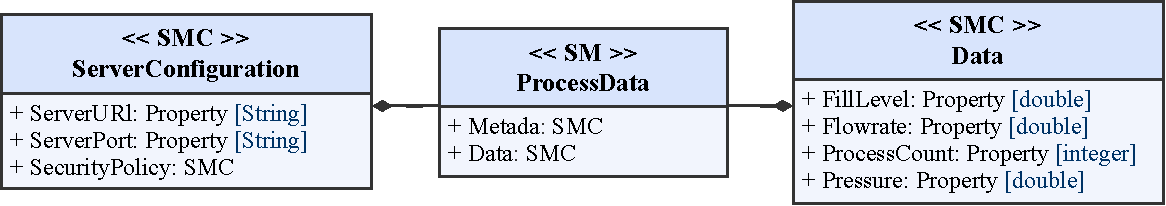
\includegraphics[width=1\textwidth]{Bilder/OPCUA/SubmodellProzessdaten.pdf}
    \caption{Submodell Prozessdaten}
    \label{fig:SubmodellProzessdaten}
\end{figure}

Das Eclipse BaSyx-Projekt stellt hierfür eine weitere Komponente bereit, die sogenannte Databridge \cite{BaSyxDatabridge}.
Diese steht, wie alle anderen Komponenten auch, als Docker-Container zur Verfügung und ermöglicht die Anbindung verschiedenster Datenquellen an eine \acs{aas}.
Sie unterstützt eine Vielzahl von Protokollen, darunter insbesondere auch \acs{opcua} oder MQTT.
Dabei dient sie als Vermittler zwischen einem Datenendpunkt und einem Submodell innerhalb der \acs{aas}.

Die Konfiguration der Databridge erfolgt über mehrere JSON-Dateien.
In einer zentralen Konfigurationsdatei werden sowohl die Datenquelle als auch die Datensenke definiert.
Außerdem können Transformatoren angegeben werden, die beispielsweise Einheitenumrechnungen oder Typkonvertierungen übernehmen.

Als Datenquelle muss der \acs{opcua} Server des Datengenerators angegeben werden, dessen Konfiguration typischerweise in einer separaten JSON-Datei erfolgt.
Darin sind sowohl die Verbindungsparameter des Servers (z.B. \acs{url} (Uniform Resource Locator) und Port) als auch die zu überwachenden Knoten anzugeben.
Wie in Abbildung \ref{fig:OPCUADatenStruktur} zu erkennen, stellt der \acs{opcua} Server die Werte hierfür in einer hierarchischen Struktur bereit, wobei jeder Knoten über einen Namespaceindex (ns) und eine NodeId (i) eindeutig adressierbar ist.

\begin{figure}[htbp]
    \centering
    % 0.88
    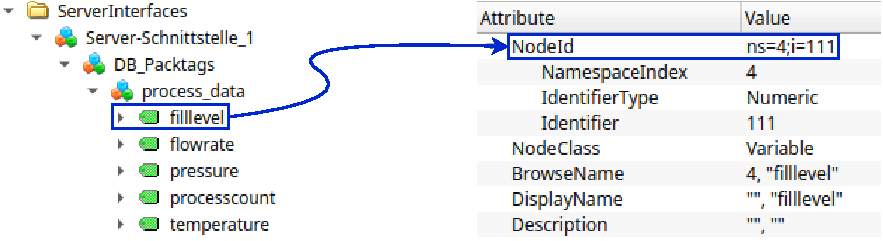
\includegraphics{Bilder/OPCUA/OPCUADaten.pdf}
    \caption{OPC UA Datenknoten}
    \label{fig:OPCUADatenStruktur}
\end{figure}

Außerdem muss der zu verwendende \acs{opcua} Client festgelegt werden.
In diesem Projekt wird Eclipse Milo eingesetzt, der auf einem Subscription-Modell basiert.
Im Gegensatz zu einem Polling-Ansatz werden hier gezielt bestimmte Knoten (Nodes) abonniert, sodass neue Werte automatisch bei Änderung übermittelt werden.

Ein Beispiel für eine entsprechende JSON-Konfiguration der Datenquelle ist in Listing~\ref{lst:jsonDatenquelle} für den Druckwert dargestellt.
Weitere optionale Parameter, wie etwa Sicherheitseinstellungen oder das Übertragungsintervall können zusätzlich angegeben werden, wurden hier jedoch zur besseren Übersicht weggelassen.

\newpage
\begin{lstlisting}[language=json, caption={Beispielhafte JSON-Konfiguration einer Datenquelle}, label={lst:jsonDatenquelle}]
{
    "uniqueId"       : "pressure",
    "nodeInformation": "ns=4;i=113",
    "serverUrl"      : "opcua-server",
    "serverPort"     : 4840,
    "pathToService"  : "milo"
}
\end{lstlisting}

Zur Anpassung der eingehenden Daten an die Struktur der Ziel-Property lassen sich verschiedene Transformatoren einsetzen.
Die Databridge unterstützt hierfür unter anderem JSONata-Ausdrücke oder JsonJacksonTransformers.
Mithilfe dieser Mechanismen können die vom \acs{opcua}-Server empfangenen Rohdaten zunächst in ein JSON-Objekt überführt und anschließend gezielt extrahiert und weiterverarbeitet werden.

Im Anschluss erfolgt die Konfiguration der Datensenke, also der Zielkomponente innerhalb der \acs{aas}.
Auch diese erfolgt über eine separate JSON-Datei, in der der Endpunkt des Submodells, der idShortPath der gewünschten Property sowie die verwendete API-Version definiert werden.
Listing~\ref{lst:jsonDatensenke} zeigt ein Beispiel einer entsprechenden Konfiguration.
Der Platzhalter \{smId\} steht dabei für die Base64-kodierte ID des Submodells Prozessdaten, wie sie in der \acs{rest}-API der \acs{aas} verwendet wird.

\begin{lstlisting}[language=json, caption={Beispielhafte JSON-Konfiguration einer Datensenke}, label={lst:jsonDatensenke}]
{
    "uniqueId"        : "Submodel/ProcessData/Pressure",
    "submodelEndpoint": "http://aas-env:8081/submodels/{smId}",
    "idShortPath"     : "Data.Pressure",
    "api"             : "DotAAS-V3"
}
\end{lstlisting}

Nach erfolgreicher Konfiguration übernimmt die Databridge die automatisierte Übertragung der \acs{opcua}-Werte in die entsprechenden Properties des Submodells.
Dieses Prinzip lässt sich nicht nur auf Prozesswerte anwenden, sondern auch zur Abbildung des Maschinenzustands oder anderer dynamischer Betriebsdaten nutzen.
Somit bildet die Databridge eine flexible und protokolloffene Lösung zur Echtzeitanbindung externer Datenquellen an eine \acs{aas}.


\subsubsection{Verarbeitung von Zeitreihendaten}
\label{sec: VerarbeitungZeitreihen}
Grundsätzlich lassen sich Zeitreihendaten auf unterschiedlichste Weise in eine \acs{aas} einbinden.
Das \acs{smt} Time Series Data \cite{SpezifikationTimeSeriesData} bietet hierfür mehrere standardisierte Lösungsansätze.
Eine Möglichkeit besteht darin, diese direkt über ein InternalSegment in der \acs{aas} zu speichern.
Diese Variante eignet sich jedoch nur für kleinere Datenmengen.
Alternativ können die Daten in Form einer Datei abgespeichert werden.
Diese können dann entweder direkt in die \acs{aas} eingebunden oder extern über ein ExternalSegment referenziert werden.
Für größere Datenmengen bietet sich die externe Speicherung an einem seperaten Ort, wie etwa einer Datenbank, an.
Diese kann über ein LinkedSegment mit der \acs{aas} verknüpft werden.

Im Folgenden wird die zuletzt genannte Option näher betrachtet.
Hierzu werden die simulierten Werte für Druck und Temperatur des Datengenerators extern in einer InfluxDB gespeichert.
Die über \acs{opcua} bereitgestellten Daten werden dabei mithilfe von Telegraf, einem leichtgewichtigen Agenten zur Datenerfassung und -weiterleitung \cite{Influx}, kontinuierlich in eine speziell für diesen Anwendungsfall angelegte Tabelle geschrieben.
InfluxDB sowie Telegraf stehen beide als Docker-Container zur Verfügung und lassen sich so nahtlos in das bestehende BaSyx-System integrieren.

Um die in der Datenbank gespeicherten Daten in die \acs{aas} einzubinden, kann das bereits genannte \acs{smt} Time Series Data verwendet werden.
Der strukturelle Aufbau ist in Abbildung \ref{fig:SMTTimeSeriesData} dargestellt.

\begin{figure}[htbp]
    \centering
    % 0.88
    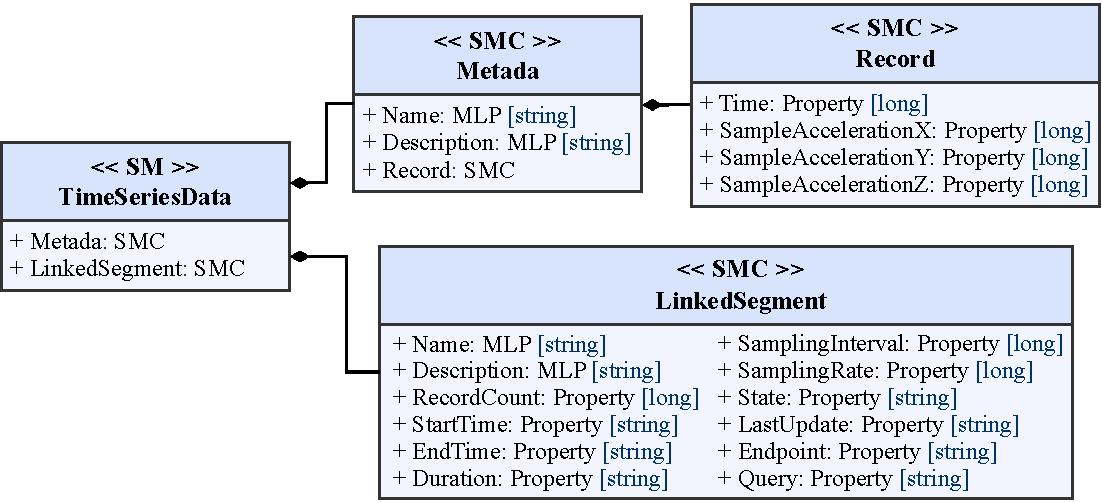
\includegraphics[width=1\textwidth]{Bilder/TimeSeries/SM_TimeSeriesData.pdf}
    \caption{SMT Time Series Data}
    \label{fig:SMTTimeSeriesData}
\end{figure}

Zuerst müssen die Metadaten eingetragen werden. 
Dazu gehören ein eindeutiger Name, eine Beschreibung sowie die Festlegung der Struktur der aufzuzeichnenden Datenpunkte in der \acs{smc} Records.
Ein Record kann mit einer Spaltenbeschreibung in einer Tabelle verglichen werden.
Er beschreibt, welche Variablen, in diesem Fall Druck und Temperatur, in einem Zeitreihen-Datensatz enthalten sind und wie diese zu interpretieren sind.

Anschließend folgt die Konfiguration des LinkedSegments. 
Dieses stellt die eigentliche Verbindung zu den extern gespeicherten Zeitreihendaten her.
Hierfür sind sowohl der Datenendpunkt als als auch die Query, mit der die gewünschten Werte ausgelesen werden sollen, zu spezifizieren.
Im vorliegenden Fall handelt es sich dabei um die Adresse des InfluxDB-Containers sowie die Abfrage, mit der die Werte für Druck und Temperatur aus der zugehörigen Tabelle extrahiert werden können.

Dabei ist zu beachten, dass der entsprechende Port der InfluxDB nach außen freigegeben ist, da andernfalls kein Zugriff durch externe Anwendungen möglich ist.
Ergänzend können weitere Metadaten angegeben werden, beispielsweise die Abtastrate (samplingRate), der durch das Segment abgedeckte Zeitraum oder ein recordCount, der die erwartete Anzahl an Einträgen innerhalb dieses Zeitfensters beschreibt.

Zur Visualisierung der Zeitreihendaten bietet das BaSyx-System eine praktische Lösung.
Über ein entsprechendes Plugin können die im Submodell Time Series Data enthaltenen Informationen direkt in der Benutzeroberfläche der AAS Web UI dargestellt werden.
Die über das LinkedSegment referenzierten Zeitreihendaten lassen sich dort in verschiedenen Diagrammen visualisieren, beispielsweise als Linien- oder Balkendiagramm.
Dadurch wird eine benutzerfreundliche Darstellung der Daten ermöglicht, ohne dass diese physisch in der \acs{aas} gespeichert werden müssen.

\subsection{KI-Modell zur Optimierung}
Im Folgenden wird ein \acs{ki}-gestütztes Konzept zur Optimierung der zustandsbasierten Prozessüberwachung innerhalb des digitalen Zwillings vorgestellt und prototypisch umgesetzt.
Ziel ist es, mithilfe maschinellen Lernens Anomalien im Betrieb des Abfüll -und Verschließmoduls der robocell frühzeitig zu erkennen und dadurch eine Grundlage für prädiktive Instandhaltungsstrategien zu schaffen.
Darüber hinaus werden die Methoden der \acs{ki} mit den Strukturen der \acs{aas} verknüpft, um eine standardisierte, interoperable Verwaltung des resultierenden Modells im Sinne der Industrie-4.0 zu ermöglichen.

\subsubsection{Konzeptidee}
Mit der fortschreitenden Digitalisierung industrieller Prozesse entstehen zunehmend umfangreiche Datenmengen, die wertvolle Informationen über den Zustand und das Verhalten eines Assets liefern. 
Dabei handelt es sich um unterschiedlichste Datenarten, etwa die Drehzahl eines Motors oder, wie im Rahmen dieser Arbeit im digitalen Zwilling abgebildet, klassische Prozessdaten wie Druck und Temperatur.
Die manuelle Analyse dieser Daten kann sich als sehr herausfordernd gestalten. Abweichungen vom Normalbetrieb sind oft schwer zu erkennen, was eine zuverlässige Zustandsüberwachung erheblich erschwert.

Ein vielversprechender Ansatz, der genau diese Problematik adressiert, ist der sogenannte Autoencoder. 
Dieser stellt eine spezielle Architektur tiefer neuronaler Netze dar und besteht typischerweise aus zwei Hauptkomponenten: einem Encoder und einem Decoder, die gemeinsam eine komprimierte, latente Repräsentation der Eingangsdaten erlernen.
\cite{Lempitsky2019}
Der prinzipielle Aufbau eines Autoencoders ist in Abbildung \ref{fig:Autoencoder} dargestellt.

% \vspace{-1em}
\begin{figure}[htbp]
    \centering
    % 0.88
    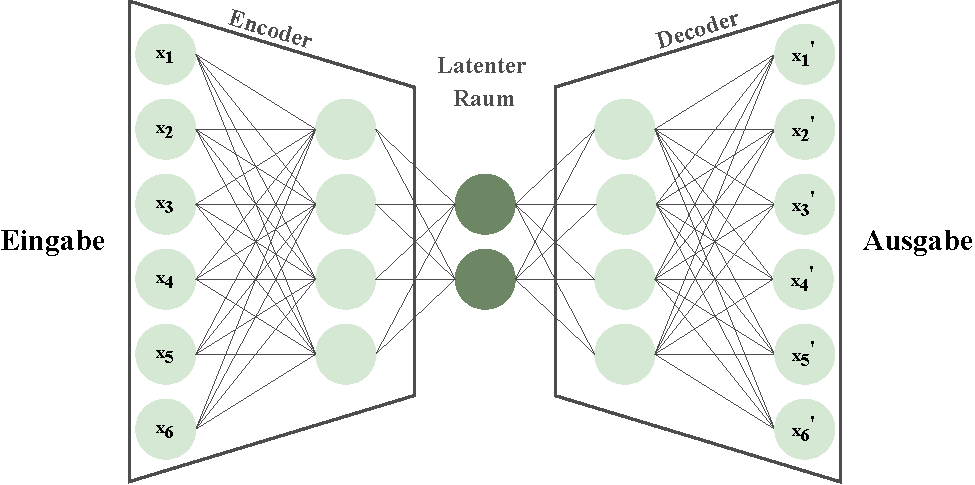
\includegraphics[width=1\textwidth]{Bilder/Autoencoder/AutoencoderModell.pdf}
    \caption{Aufbau eines Autoencoders}
    \label{fig:Autoencoder}
\end{figure}

Der Encoder besteht aus mehreren Schichten, die die Eingabedaten schrittweise in eine komprimierte Form überführen. Dabei erfolgt eine Dimensionsreduktion, das heißt, die Daten werden im Verlauf auf weniger Dimensionen verdichtet. 
Das Ziel ist es, die für die Rekonstruktion wesentlichen Merkmale zu extrahieren und irrelevante Informationen zu filtern.
Der dabei entstehende latente Raum bildet die am stärksten komprimierte Repräsentation der Daten ab und dient als Ausgangspunkt für den Decoder.
Dieser übernimmt die Aufgabe, die komprimierte Darstellung wieder in die ursprüngliche Eingabe zu rekonstruieren. 
Auch er besteht aus mehreren Schichten, die die Daten schrittweise dekomprimieren.
Zur Bewertung der Leistungsfähigkeit des Autoencoders wird die resultierende Ausgabe mit der ursprünglichen Eingabe verglichen. 
Die Differenz zwischen beiden wird als Rekonstruktionsfehler bezeichnet. \cite{Autoencoder}

Autoencoder eignen sich hervorragend zur Erkennung von Anomalien in Zeitreihendaten, insbesondere im Rahmen des unüberwachten Lernens.
Klassische Autoencoder werden dabei ausschließlich mit Daten aus dem Normalbetrieb trainiert.
Dabei lernt das Modell, typische Muster zu erkennen und ist in der Lage, normale Betriebszustände zuverlässig zu rekonstruieren.
Weichen neue Eingangsdaten deutlich vom erlernten Schema ab, gelingt die Rekonstruktion nicht mehr vollständig.
Dies führt zu einem erhöhten Rekonstruktionsfehler, der als Indikator für eine potenzielle Anomalie gewertet werden kann.

\subsubsection{Prototypische Umsetzung}
Für die prototypische Umsetzung des Autoencoders wird die Programmiersprache Python verwendet.
Als Datengrundlage dienen die simulierten Temperaturverläufe, die mithilfe des Datengenerators erzeugt und, wie auch in Kapitel \ref{sec: VerarbeitungZeitreihen} beschrieben, in einer InfluxDB gespeichert sind.
Um diese vorzubereiten, wird ein Python-basierter InfluxDB-Client verwendet, der über ein \acs{api}-Token sowie die \acs{url} des Datenbanksystems mit der Datenquelle kommuniziert.
Die relevanten Temperaturdaten werden über eine gezielte Abfrage aus der Datenbank extrahiert.
In dieser Umsetzung wird dabei ein Zeitraum von 7 Tagen betrachtet.

Die extrahierten Daten lassen sich anschließend mit NumPy in ein geeignetes Array-Format überführen und in Sequenzen unterteilen, um sie für das Training des Autoencoders vorzubereiten.
Dabei werden Zeitfenster mit einer Länge von 30 Werten bei einer Abtastrate von 1 Hz gebildet, was einem Zeitraum von 30 Sekunden entspricht.
Diese Fenstergröße wird gewählt, da relevante Veränderungen im Prozessverlauf typischerweise innerhalb kurzer Zeiträume auftreten.
Abschließend müssen die Sequenzen in einen Tensor umgewandelt werden. 
In diesem Fall handelt es sich um einen zweidimensionalen Tensor, bei dem jede Zeile eine Zeitfenster-Sequenz mit 30 Temperaturwerten enthält.

Im Anschluss an die Datenvorbereitung muss der Autoencoder konfiguriert werden. 
Dies erfolgt mit dem Deep-Learning-Framework PyTorch \cite{PyTorch}. 
In dieser Umsetzung wird ein einfaches Modell verwendet. 
Der Encoder ist so aufgebaut, dass er die Eingabesequenz mit 30 Temperaturwerten zunächst auf 5 Neuronen reduziert und anschließend auf 2 Neuronen verdichtet. 
Diese beiden Neuronen bilden den latenten Raum. 
Der Decoder ist spiegelbildlich aufgebaut, erweitert die Darstellung aus dem latenten Raum zunächst wieder auf 5 Neuronen und generiert schließlich 30 Ausgabewerte, die der ursprünglichen Eingabesequenz entsprechen.

Nach der Konfiguration des Autoencoders folgt das Training mit einer festgelegten Anzahl an Epochen. 
Dabei werden dem Modell die zuvor definierten Tensoren mit den Zeitfenster-Sequenzen als Eingabe übergeben. 
Die Rekonstruktion erfolgt für alle Sequenzen parallel. 
Anschließend wird die mittlere quadratische Abweichung (MSE) zwischen Eingabe und Ausgabe berechnet. 
Dieser Fehlerwert dient als Grundlage für die Anpassung der Modellparameter, beispielsweise durch Backpropagation. 
Der Vorgang wird iterativ über alle Epochen hinweg wiederholt, um die Genauigkeit des Modells sukzessive zu optimieren.

Das fertig trainierte Modell kann anschließend zur Erkennung von Anomalien in neuen Temperaturdaten eingesetzt werden. 
Diese Daten sind analog zu den Trainingsdaten aufgebaut, enthalten jedoch gezielt eingefügte Ausreißer bzw. Unregelmäßigkeiten. 
Während der Ausführung des Autoencoders muss für jede Sequenz der Rekonstruktionsfehler berechnet werden, der die durchschnittliche Abweichung zwischen den Eingabewerten und den rekonstruierten Ausgabewerten beschreibt.
Um Anomalien zu identifizieren, kann dieser Fehler mit einem definierten Schwellenwert verglichen werden, beispielsweise dem 95. Perzentil der Fehlerverteilung oder dem Mittelwert zuzüglich des Zweifachen der Standardabweichung. 
Überschreitet der Rekonstruktionsfehler diesen Wert, so wird die gesamte Sequenz, also das vollständige Zeitfenster mit 30 Werten, als Anomalie klassifiziert.

\subsubsection{Verwaltung der Metadaten in der \acs{aas}}
\acs{ki}-Modelle lassen sich als digitale Assets betrachten, da sie, analog zu physischen Komponenten, über einen eigenen Lebenszyklus verfügen.  
Für deren standardisierte und interoperable Verwaltung bietet sich die Integration in einen digitalen Zwilling an.  
Im Folgenden wird daher gezeigt, wie das zuvor entwickelte \acs{ki}-Modell zur Anomalieerkennung mithilfe der \acs{aas} abgebildet und verwaltet werden kann.

Für die standardisierte Beschreibung kann das \acs{smt} AIModelNameplate \cite{SpezifikationAIModelNameplate} eingesetzt werden. 
Es erfüllt eine vergleichbare Funktion wie das digitale Typenschild für physische Assets und enthält zentrale Metadaten zur Identifikation sowie Dokumentation des Modells über dessen gesamten Lebenszyklus hinweg.

Zu den abbildbaren Informationen zählen beispielsweise die \acs{url} des Modells, der Speicherort, die Versionsnummer sowie die Art des Trainingsverfahrens. 
Darüber hinaus lassen sich auch die Ein- und Ausgänge des Modells über entsprechende \acsp{smc} spezifizieren. 
Hierzu gehören unter anderem Angaben zur Art der Ein- bzw. Ausgabedaten sowie deren Struktur und Dimension. 
Im Fall des hier eingesetzten Autoencoders ist der Eingabetyp beispielsweise, wie zuvor beschrieben, eine Sequenz mit einer Dimension von 30.

Eine weitere zentrale Komponente bildet die \acs{smc} Details, in der technische Informationen wie das verwendete Framework (PyTorch), die Programmiersprache (Python) sowie die Dateiendung des gespeicherten Modells (z. B. .pt oder .onnx) dokumentiert werden. 
Ergänzend können auch Abhängigkeiten hinterlegt werden, beispielsweise in Form einer referenzierten Textdatei, die alle benötigten Python-Bibliotheken aufführt.

Das Submodell bietet außerdem die Möglichkeit, unterstützende Visualisierungen einzubinden. 
Dies können beispielsweise Grafiken zur Modellarchitektur oder Diagramme zum Trainingsverlauf sein, die direkt in Python generiert werden können. 
Solche Visualisierungen können entweder als Dateien direkt in die \acs{smc} Plots eingebettet oder über externe Referenzen verlinkt werden.

Nicht zuletzt enthält das AIModelNameplate eine Verknüpfung zu einem weiteren Submodell, das mit dem \acs{smt} AIDataset \cite{SpezifikationAIDataset} realisiert wird.
Dieses dient der strukturierten Beschreibung der für das Modelltraining verwendeten Daten.
Obwohl das \acs{smt} primär für gelabelte Datensätze ausgelegt ist, lässt es sich auch zur Beschreibung synthetisch erzeugter Daten einsetzen, wie im vorliegenden Fall des durch den Datengenerator erzeugten Temperaturdatensatzes.

Die wichtigsten Elemente umfassen, analog zum AIModelNameplate, zentrale Metainformationen wie die \acs{url}, die Versionsnummer und den Speicherort des Datensatzes.
Darüber hinaus ermöglicht die \acs{smc} SizeInformation eine strukturierte Angabe zur Datenmenge, etwa zur Anzahl der Datenpunkte in Trainings-, Validierungs- und Testdatensatz, zur Gesamtdatenmenge sowie zum Verhältnis ihrer Aufteilung.
Weitere Elemente zur Beschreibung gelabelter bzw. realer Datensätze sind ebenfalls Teil des Submodells, werden im Kontext des hier verwendeten unüberwachten Lernens mit synthetisch erzeugten Daten jedoch nicht berücksichtigt.

Für die Beschreibung der Modellbereitstellung kann ergänzend das \acs{smt} AIDeployment \cite{SpezifikationAIDeployement} eingesetzt werden, das unter anderem Angaben zu Hard- und Softwareanforderungen, Bereitstellungsoptionen, Überwachungsmechanismen sowie zur Leistungsbewertung enthält.
Im Rahmen der prototypischen Umsetzung besteht hierfür jedoch kein Bedarf, weshalb dieses Submodell an dieser Stelle lediglich der Vollständigkeit halber erwähnt wird.

\subsection{Anwendungsfall Digitaler Produktpass}
Im Kontext steigender Anforderungen an Nachhaltigkeit und Transparenz entlang des gesamten Produktlebenszyklus eines Assets gewinnt der \acs{dpp} zunehmend an Bedeutung. 
Der Fokus dieses Anwendungsfalls liegt auf zwei zentralen Aspekten: der Abbildung des \acs{pcf} sowie der technischen Umsetzung der Zugriffsrechte auf die im \acs{dpp} enthaltenen Daten.

Der \acs{pcf} beschreibt die Summe aller Treibhausgasemissionen, ausgedrückt in CO\textsubscript{2}-Äqui\-valenten, die entlang des Lebenszyklus eines Produkts entstehen \cite{PCF}. 
Seine Bedeutung zeigt sich auch in der EU-Batterieverordnung \cite{EUVerordnung}, die die Einführung eines digitalen Batteriepasses vorschreibt, der die erste konkrete Umsetzung eines \acs{dpp} darstellt und daher als Ausgangspunkt für weitere Branchen wie den Maschinen- und Anlagenbau dient.
Darin wird unter anderem die verpflichtende Angabe des \acs{pcf}, insbesondere für die Phasen Material, Produktion und die Gesamtbetrachtung (Cradle to Gate) gefordert, welche im Rahmen dieses Anwendungsfalls exemplarisch umgesetzt werden. 
Für weiterführende Lebenszyklusphasen wie die Nutzung ist die Angabe derzeit noch nicht vorgeschrieben.

Die technische Umsetzung orientiert sich an dem vom ZVEI vorgestellten Konzept des \acs{dpp40}, das unter anderem gemeinsam mit der \acs{idta} im Rahmen eines \acs{pcf}-Showcases auf einer Website demonstriert wird \cite{PCFShowcas}.
Aufbauend auf diesem Konzept wird gezeigt, wie ein \acs{dpp} mithilfe der \acs{aas} modelliert und prototypisch realisiert werden kann.

Konkret wird der digitale Zwilling des Abfüll- und Verschließmoduls der robocell um ein Submodell zur Abbildung des \acs{pcf} erweitert. 
Der Fokus liegt auf der exemplarischen Aggregation von CO\textsubscript{2}-Daten aus Zulieferkomponenten, um den \acs{pcf} des Moduls zu berechnen. 
Ergänzend wird demonstriert, wie sich Zugriffsrechte auf die im \acs{dpp} enthaltenen Informationen mithilfe der Eclipse BaSyx-Plattform umsetzen lassen.

\subsubsection{Umsetzung mit dem Teilmodell Carbon Footprint}
Zur exemplarischen Abbildung und dynamischen Berechnung des \acs{pcf} der Gesamtmaschine wird das von der \acs{idta} spezifizierte \acs{smt} \acs{cf} \cite{SpezifikaitonPCF} eingesetzt.  
Dieses Template definiert eine standardisierte Struktur zur Erfassung von CO\textsubscript{2}-Äquivalenten entlang des Produktlebenszyklus.  
Es unterscheidet zwischen dem \acs{pcf} und dem Transport Carbon Footprint (TCF), wobei im Rahmen dieses Anwendungsfalls ausschließlich der \acs{pcf} betrachtet wird.

Das \acs{smt} gibt die Struktur des \acs{pcf} in Form einer \acs{smc} vor.  
Diese Sammlung enthält standardisierte Elemente wie den CO\textsubscript{2}-Wert, die zugehörige Lebenszyklusphase, die verwendete Berechnungsmethode sowie den Gültigkeitszeitraum.
Wie bereits zuvor beschrieben, liegt der Fokus auf den Lebenszyklusphasen Material, Produktion und Cradle to Gate.  
Für jede dieser Phasen empfiehlt es sich, eine eigene \acs{smc} gemäß der Submodellspezifikation zu erstellen.  
Diese Sammlungen dienen als Basis für die spätere Aggregation der \acs{pcf}-Werte der Gesamtmaschine und werden im weiteren Verlauf dynamisch mit Werten befüllt.

Für die exemplarische Berechnung des \acs{pcf} wurde eine Auswahl an Steuerungskomponenten festgelegt, die in der robocell verbaut sind.  
Diese Auswahl beschränkt sich auf Siemens-Komponenten, darunter beispielsweise eine CPU sowie Ein- und Ausgangsmodule.  
Die Komponenten wurden als Typ-1-\acs{aas} zur Verfügung gestellt, wobei jede \acs{aas} ein eigenes Submodell gemäß des \acs{smt} \acs{cf} enthält.

Um diese in die \acs{pcf}-Berechnung einzubeziehen, können sie direkt im \acs{cf}-Submodell der robocell referenziert werden. 
In diesem Anwendungsfall erfolgt dies über eine \acs{sml}, in der die Komponenten als Entities unter Angabe ihrer jeweiligen globalAssetId eingebunden sind. 
Alternativ wäre auch eine Referenzierung direkt über das \acs{bom}-Submodell möglich.

Für die dynamische Berechnung müssen sowohl die \acs{aas} der robocell als auch die zugehörigen Komponenten-\acs{aas} in einer Laufzeitumgebung verfügbar sein. 
Die Bereitstellung erfolgt über die Eclipse BaSyx-Plattform.
Zur Benutzerinteraktion wird das bestehendes Vue.js-Plugin für den Carbon Fooprint der AAS Web UI genutzt.
Dieses wird im Rahmen dieses Anwendungsfalls um eine Schaltfläche zur Initialisierung der Aggregation erweitert.

Die Aggregationslogik ist als eigenständiger, Node.js-basierter Microservice mit einer Web-API implementiert. 
Diese wertet die Komponenten-\acs{aas} aus, berechnet die aggregierten Werte für die zuvor definierten Lebenszyklusphasen und schreibt diese in das \acs{cf}-Submodell der Haupt-AAS der robocell zurück. 
Die Auslösung des Microservice erfolgt über die Schaltfläche im erweiterten Plugin.

Alternativ wäre auch eine clientseitige Berechnung direkt im \acs{cf}-Plugin denkbar. 
In der vorliegenden Umsetzung liegt die gesamte Aggregationslogik jedoch zentral und serverseitig im Microservice. 
Der Ablauf ist in Abbildung \ref{fig:SequenzdiagrammPCF} als Sequenzdiagramm dargestellt.

% \newpage
% \begin{figure}[htbp]
%     \centering
%         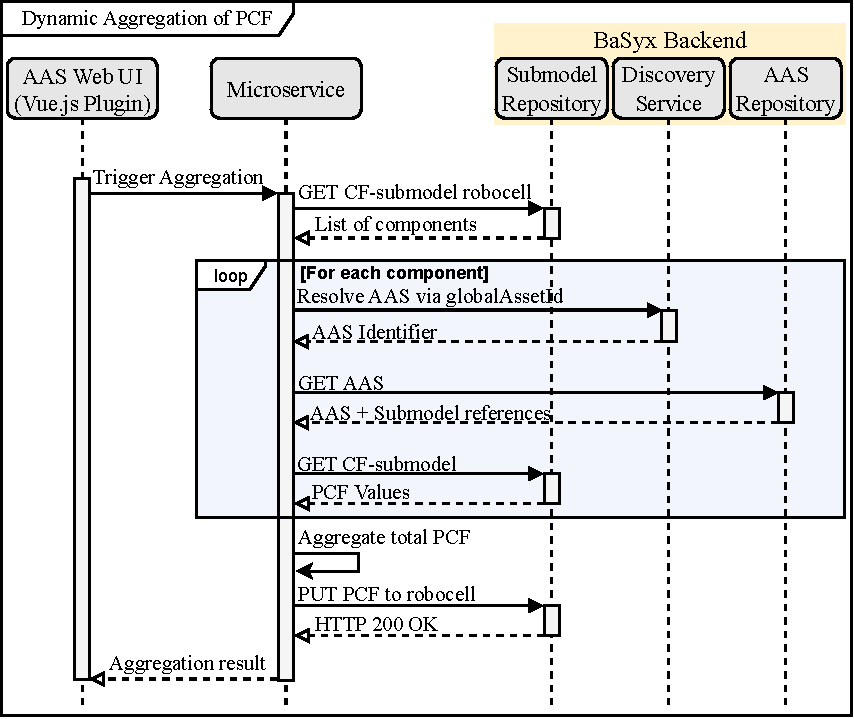
\includegraphics[width=1\textwidth]{Bilder/DPP/PCF_Aggregation_SmallLine.pdf}
    
%     \caption{Sequenzdiagramm zur Aggregation des PCF}
%     \label{fig:SequenzdiagrammPCF}
% \end{figure}

% !!!! Das und das Bidl vielleicht schon Ergebnisse !!!!
Der Microservice nutzt die \acs{rest}-Schnittstelle des Submodel Repositories der AAS Environment, um zunächst alle in der \acs{aas} der robocell hinterlegten Komponenten auszulesen. 
Mithilfe des Discovery Service werden auf Basis ihrer globalAssetIds die zugehörigen Komponenten-\acs{aas} identifiziert und anschließend vom AAS Repository abgerufen.
Für jede dieser Komponenten wird geprüft, ob ein \acs{cf}-Submodell vorhanden ist. 
Falls dies zutrifft, wird das Submodell ausgelesen und die enthaltenen Werte extrahiert.

Aus den ermittelten Einzelwerten berechnet der Microservice schließlich die aggregierten CO\textsubscript{2}-Äquivalente für die Phasen Produktion, Material sowie Cradle to Gate. 
Die berechneten Werte werden abschließend in das \acs{cf}-Submodell der Haupt-\acs{aas} der robocell geschrieben und stehen dort strukturiert zur Verfügung.

\subsubsection{Zugriffsrechte und Datensicherheit}

Die kontrollierte Bereitstellung der im \acs{dpp} enthaltenen Informationen ist essenziell, insbesondere im Hinblick auf Datenschutz, regulatorische Vorgaben sowie den Schutz geistigen Eigentums.  
Wie in Kapitel~\ref{sec: Sicherheit} beschrieben, sieht die Security-Spezifikation der \acs{idta} hierfür die Nutzung eines attributbasiertes Zugriffskontrollmodell (\acs{abac}) vor.

Da die \acs{abac}-Funktionalität in aktuellen Referenzimplementierungen wie dem AASX Server Blazor oder Eclipse BaSyx jedoch noch nicht vollständig verfügbar ist, wird im Rahmen dieses Anwendungsfalls exemplarisch ein rollenbasiertes Zugriffskontrollmodell (\acs{rbac}) eingesetzt, wie es von der Eclipse BaSyx-Plattform unterstützt wird.  
Die Zugriffskontrolle erfolgt dabei durch die Zuweisung spezifischer Berechtigungen an vordefinierte Rollen, denen wiederum Benutzer oder technische Clients zugeordnet werden.

Zur Umsetzung von Authentifizierung und Autorisierung wird der Open-Source Identity Provider Keycloak verwendet \cite{Keycloak}.  
Dieser ermöglicht die zentrale Verwaltung von Benutzern, Rollen und Clients und unterstützt eine tokenbasierte Zugriffskontrolle auf Basis von \acsp{jwt}.  
Keycloak steht dabei als Docker-Container zur Verfügung und kann nahtlos in die BaSyx-Systemarchitektur integriert werden.

Im ersten Schritt muss ein dediziertes Realm eingerichtet werden, das als gekapselte Umgebung für alle projektbezogenen Identitäten dient.  
Innerhalb dieses Realms lassen sich sowohl Benutzerkonten als auch Rollen definieren, wobei die Zuweisung über sogenannte Role Mappings erfolgt.  
Ein Benutzer kann dabei einer oder mehreren Rollen gleichzeitig zugewiesen sein.

Jedes Benutzerkonto verfügt über einen eindeutigen Benutzernamen sowie ein initiales Passwort zur Authentifizierung.  
Zur Erhöhung der Sicherheit kann dieses Passwort als temporär markiert werden, wodurch der Benutzer bei der ersten Anmeldung zu einer Änderung gezwungen wird.  
Darüber hinaus bietet Keycloak ebenfalls die Möglichkeit, sogenannte Required Actions zu definieren, etwa zur E-Mail-Verifizierung oder zur erzwungenen Passwortänderung beim nächsten Login.  
Dies erlaubt eine flexible Anpassung des Authentifizierungsprozesses an projektspezifische Sicherheitsanforderungen.

Im Rahmen dieses Anwendungsfalls werden exemplarisch folgende Benutzer eingerichtet:

\begin{itemize}[noitemsep, leftmargin=*, label=\textbullet]
  \item \makebox[6cm][l]{\textbf{groninger.meyer}} (Rolle: \textit{Groninger-Mitarbeiter})
  \item \makebox[6cm][l]{\textbf{customer.doe}} (Rolle: \textit{Kunde})
  \item \makebox[6cm][l]{\textbf{technician.john}} (Rolle: \textit{Service-Techniker})
\end{itemize}

Neben der Verwaltung menschlicher Benutzer unterstützt Keycloak auch die Administration technischer Clients, die z.B. maschinelle Anwendungen oder externe Systeme repräsentieren.  
Die Authentifizierung erfolgt in der Regel über eine Kombination aus eindeutiger Client-ID und einem geheimen Schlüssel (Client Secret) gemäß dem OpenID Connect-Protokoll.  
Für jeden Client kann optional ein Service Account aktiviert werden, der als technisches Benutzerkonto agiert und - analog zu realen Benutzern - mit spezifischen Rollen ausgestattet wird.  
Dies ermöglicht eine differenzierte Zugriffsteuerung auch für automatisierte Systemzugriffe.

Die Rechtevergabe innerhalb von Eclipse BaSyx erfolgt rollenbasiert über externe Konfigurationsdateien (i.~d.~R. im JSON-Format).  
Darin wird definiert, welche Rollen welche Berechtigungen (z.~B. READ, WRITE, DELETE ) auf bestimmte Elemente wie \acs{aas}, Submodelle oder Concept Descriptions erhalten.  
Für generische Regeln kann der Platzhalter \texttt{*} verwendet werden, um z.~B. den Zugriff auf alle Submodelle einer BaSyx-Komponente zu gewähren.  
Die AAS Web UI benötigt keine eigene \acs{rbac}-Datei, sondern orientiert sich an den Konfigurationen der angebundenen Services.

Im Rahmen dieses Szenarios erhält die Rolle Groninger-Mitarbeiter vollständige Zugriffsrechte auf alle Submodelle des \acs{dpp}, während die Rolle Kunde ausschließlich Leserechte auf ausgewählte Submodelle (z.B. Typenschild oder Technische Daten) besitzt.  
Die Rolle Service-Techniker hingegen verfügt über Lese- und Schreibrechte auf wartungsrelevante Submodelle (z.\,B. Wartung, Kontrollkomponente), jedoch ohne Zugriff auf das \acs{pcf}-Submodell, das für diese Rolle nicht vorgesehen ist.  
Eine exemplarische \acs{rbac}-Konfiguration der Rolle Groninger-Mitarbeiter für die AAS Environment ist in Listing~\ref{lst:groningerMitarbeiterRBAC} dargestellt.

\begin{lstlisting}[language=json, caption={RBAC-Konfiguration für die Rolle Groninger-Mitarbeiter}, label={lst:groningerMitarbeiterRBAC}]
{
    "role": "groninger-employee",
    "action": ["CREATE", "READ", "UPDATE", "DELETE"],
    "targetInformation": {
        "@type": "submodel",
        "submodelIds": "*",
        "submodelElementIdShortPaths": "*"
    }
}
\end{lstlisting}

Eine Möglichkeit, die im \acs{dpp} enthaltenen Informationen einzusehen, bietet die AAS Web UI. 
Ist \acs{rbac} aktiviert, wird der Benutzer beim Aufruf der Oberfläche zur Keycloak-Anmeldeseite weitergeleitet.  
Nach erfolgreicher Authentifizierung erhält der registrierte Client (AAS Web UI) ein Zugriffstoken, das die Rolleninformationen des Nutzers enthält.  
Dieses Token wird im Hintergrund an die angebundenen BaSyx-Komponenten (z.\,B. AAS Environment, Registry) weitergegeben.  
Die Entscheidung über die tatsächliche Zugriffsberechtigung trifft dabei nicht die AAS Web UI, sondern der jeweilige Service, indem er die im Token enthaltenen Rollen gegen die hinterlegten RBAC-Regeln prüft.

Alternativ ist auch ein direkter Zugriff über die \acs{api} möglich, etwa durch technische Clients oder externe Anwendungen.  
In diesem Fall muss das Zugriffstoken aktiv über den Token-Endpunkt des entsprechenden Realms bei Keycloak angefordert und anschließend im HTTP-Header der Anfrage übermittelt werden.  
Die Autorisierung erfolgt analog zur Web-Oberfläche durch die jeweiligen BaSyx-Komponenten basierend auf den Rollen im Token und den definierten \acs{rbac}-Konfigurationen.

\subsection{Anwendungsfall automatisierte Generierung von AAS}
Ziel dieses Anwendungsfalls ist es, den Prozess der automatisierten Generierung einer \acs{aas} exemplarisch darzustellen. 
Hierzu wird im ersten Schritt ein unternehmensspezifisches \acs{smt} erstellt, das anschließend in ein Typ-Submodell überführt wird.
Dieses bildet die Grundlage für die automatisierte Erstellung eines Instanz-Submodells, das mit konkreten Daten befüllt, in eine \acs{aas} eingebettet und schließlich in das BaSyx-System integriert wird.

\subsubsection{Arbeiten mit Submodel Templates}
\label{chap:ErstellenvonSubmodelTemplates}
Für die automatisierte Generierung einer \acs{aas} ist eine konsistente Submodellstruktur erforderlich, die sich aus wiederverwendbaren Vorlagen ableiten lässt.
Im vorliegenden Anwendungsfall dient das standardisierte \acs{smt} Technische Daten \cite{SpezifikaitonTechnischeDaten} als Ausgangspunkt. 
Dieses definiert eine generische Struktur zur Beschreibung technischer Merkmale, gegliedert in Kategorien (\acsp{smc}) wie Generelle Informationen, Technische Informationen oder Produktklassifikation. 
Es bildet somit den semantischen Rahmen, enthält jedoch zunächst keine konkreten Ausprägungen.

Auf Unternehmensebene kann das generische Template an spezifische Anforderungen angepasst werden, beispielsweise für einen bestimmten Maschinentyp wie die robocell.
Branchenspezifische Varianten sind grundsätzlich ebenfalls denkbar, werden in diesem Anwendungsfall jedoch nicht weiter betrachtet.

Die Anpassung kann mithilfe des Package Explorers erfolgen.
Über diesen lässt sich das standardisierte \acs{smt} importieren und anschließend gezielt erweitern.
So können etwa produktspezifische Anforderungen, wie Umgebungsbedingungen oder der Verarbeitungsbereich, mithilfe geeigneter Submodellelemente ergänzt werden.
Das resultierende unternehmensspezifische Template erhält eine eigene semanticId, bleibt jedoch zusätzlich mit der ursprünglichen semanticId des generischen Templates verknüpft, um die Rückverfolgbarkeit zur standardisierten Vorlage sicherzustellen.

Anschließend kann aus dem angepassten Template ein Typ-Submodell abgeleitet werden, das nicht nur die Struktur, sondern bereits allgemeingültige Merkmale einer Produktgruppe enthält, beispielsweise den Einsatzort oder die maximal zulässige Umgebungstemperatur.
Dieses Typ-Submodell dient als Vorlage für die spätere Erstellung konkreter \acs{aas}-Instanzen, die anschließend mit produktspezifischen Werten wie einer Seriennummer vervollständigt werden.
Die Verbindung zur ursprünglichen sowie zur unternehmensspezifischen Template-Struktur wird dabei über entsprechende semanticId-Verknüpfungen beibehalten.


\subsubsection{Automatisiertes Befüllen mit strukturierten Daten}
Nach der Erstellung eines Typ-Submodells stellt sich die Frage, wie dieses effizient mit konkreten Produktinformationen befüllt und anschließend in eine vollständige \acs{aas}-Instanz überführt werden kann.

In der industriellen Praxis liegen die benötigten Daten meist bereits strukturiert in bestehenden IT-Systemen wie \acs{plm}- oder \acs{erp}-Lösungen vor.
Da eine direkte Systemintegration im Rahmen dieser Arbeit nicht realisierbar ist, wird der Prozess exemplarisch anhand vordefinierter Beispieldaten demonstriert.
Diese Daten enthalten typische technische Merkmale, wie sie auch in realen Unternehmenssystemen vorzufinden sind, und bilden die Grundlage für die automatisierte Erstellung eines Instanz-Submodells.

Die technische Umsetzung erfolgt über ein Skript, das diese Daten automatisiert in die vorgegebene Submodellstruktur überträgt und anschließend in eine neu erzeugte \acs{aas}-Instanz einbettet.
In diesem Projekt wird dazu die serverseitige JavaScript-Laufzeitumgebung Node.js \cite{nodejs} verwendet, da sie eine einfache Verarbeitung von \acs{json}-Daten sowie eine unkomplizierte Kommunikation mit \acs{rest}-Schnittstellen ermöglicht. 

Als Basis werden drei zentrale \acs{json}-Komponenten benötigt:

\begin{enumerate}[noitemsep, leftmargin=*, label=\textbf{\arabic*.}]
    \item \textbf{Datenquelle:} Technische Produktinformationen
    \item \textbf{Submodell-Vorlage:} Struktur und Semantik des Submodells
    \item \textbf{AAS-Vorlage:} Aufbau und Struktur der \acs{aas}-Instanz
\end{enumerate}

Die Datenquelle ist hierarchisch aufgebaut und enthält verschachtelte Schlüssel-Wert-Paare. 
Jeder Schlüssel entspricht einem idShort-Wert eines Elements innerhalb der Submodell-Vorlage. 
Diese wiederum ist so konzipiert, dass Platzhalter an den relevanten Stellen eingefügt sind, die bei der Skriptausführung mit den zugehörigen Werten aus der Datenquelle ersetzt werden.

Nach der Befüllung des Instanz-Submodells mit konkreten Werten muss dieses in eine neu erzeugte \acs{aas}-Instanz eingebunden werden.
Die zugrunde liegende \acs{aas}-Vorlage definiert die grundlegende Struktur in einer separaten Datei, enthält jedoch noch keine spezifischen Identifikatoren, wie beispielsweise die eindeutige ID der \acs{aas} oder des zugehörigen Assets.
Um diese hinzuzufügen, können während der Skriptausführung zufällig generierte UUID-Werte (Universally Unique Identifier) an den entsprechenden Stellen in die Vorlage eingefügt werden.

Im letzten Schritt erfolgt die Bereitstellung der AAS-Instanz innerhalb des Eclipse BaSyx-Systems. 
Hierzu kann die \acs{aas} sowie das zugehörige Submodell, analog zur Möglichkeit~C \acs{rest}-API aus Kapitel~\ref{sec:bereitstellungAAS}, eingebunden und registriert werden.
